\label{compreensao_sae}

O sistema \acrshort{SAE} foi desenvolvido para automatizar a gestão do Programa Nacional de Assistência Estudantil da Universidade (PNAES), que está em vigor conforme preconiza o Decreto n. 7.234, de 19 de julho de 2010. 
Este decreto visa ampliar as condições de permanência dos jovens na educação superior federal; minimizar os efeitos das desigualdades sociais e regionais na permanência e conclusão da educação superior; reduzir as taxas de retenção e evasão; e contribuir para a promoção da inclusão social pela educação.

Nesse sentido, o sistema \acrshort{SAE} oferece funcionalidades para fazer a gestão da Avaliação Socioeconômica para acesso aos PNAES e destina-se aos estudantes regularmente matriculados em disciplinas de cursos presenciais de graduação e pós-graduação (mestrado e doutorado) da Universidade.

Para efetivação da política PNAES da Universidade, os estudantes são categorizados de acordo com a sua situação socioeconômica em: Participantes dos Programas de Assistência Estudantil (PPAES), condição considerada insuficiente para a manutenção do estudante na Universidade; e Não Participantes dos Programas de Assistência Estudantil (N-PPAES), situação socioeconômica considerada suficiente para a manutenção do estudante na Universidade. Assim, os estudantes classificados como Participantes dos Programas de Assistência Estudantil (PPAES) caracterizam perfil de vulnerabilidade socioeconômica.

Para que o aluno possa participar do processo de avaliação socioeconômica, a \acrshort{UnB} disponibiliza o acesso público ao sistema \acrshort{SAE} (pela url http://www.saeweb.unb.br) para que o aluno possa realizar o preenchimento dos formulários do estudo socioeconômico. Posteriormente, se aprovado, o aluno precisa entregar os documentos solicitados pelo programa. Além desses passos, é exigido entrevistas com os alunos pré-aprovados nos benefícios.

Entre os principais programas de assistência estudantil, destacam-se:

\begin{itemize}

\item Auxílio-Alimentação. O Auxílio-Alimentação consiste no repasse mensal de recurso em forma de pecúnia para os estudantes identificados em situação de vulnerabilidade socioeconômica.

\item Bolsa Permanência para Estudantes de Graduação. Tem o objetivo de minimizar as desigualdades sociais e contribuir para a permanência e a diplomação dos estudantes de graduação da Universidade de Brasília que se encontram em situação de vulnerabilidade socioeconômica. 

\item Moradia Estudantil. Oferece moradia temporária aos estudantes em situação de vulnerabilidade socioeconômica, prioritariamente aos oriundos de famílias que residem fora do Distrito Federal ou provenientes de regiões de difícil acesso.

\end{itemize}

Para avaliação socioeconômica, são considerados vários dados informados pelo aluno, como a renda familiar, profissão/ocupação e nível de escolaridade do(s) mantenedor(es) ou cônjuge, grupo familiar (o número de membros declarados no formulário socioeconômico e
comprovados mediante documentação), local de moradia do estudante e da família, despesas da família com aluguel ou com financiamento da casa própria, pessoas diagnosticadas com doenças crônicas ou degenerativas e pessoas com deficiência.

O primeiro resultado do estudo socioeconômico é liberado para consulta para que os alunos possam verificar sua classificação. Eventuais recursos aos resultados do processo a seletivo poderão alterar a classificação inicial dos candidatos, após análise do Serviço Social do SPS/DDS. No decorrer do semestre letivo, havendo alteração na situação socioeconômica, o estudante poderá impetrar recurso solicitando reavaliação do estudo. 

O estudante que desejar interpor recurso ao resultado da avaliação socioeconômica e da moradia estudantil deverá solicitar em formulário próprio do SPS/DDS em até até 30 dias contados a partir da divulgação do resultado. A análise do recurso deve ser analisado no prazo máximo de 15 (quinze) dias úteis após a data de interposição.

Ao final do processo, os alunos beneficiados terão acesso aos Programas mediante assinatura do Termo de Concessão junto ao Serviço de Programas de Desenvolvimento Social (SPS/DDS) localizado no Campus onde está matriculado. O referido termo deverá ser assinado no semestre da concessão de acordo com o prazo previsto em cada Programa. A concessão e a manutenção dos Programas de Assistência Estudantil estarão condicionadas a vinculação do estudante à Universidade de Brasília, sendo pessoal, temporária e intransferível.

A Figura~\ref{fig:ER_SAE} mostra o modelo entidade relacionamento do \acrshort{SAE}.

\begin{figure}[ht]
\advance\leftskip-4cm
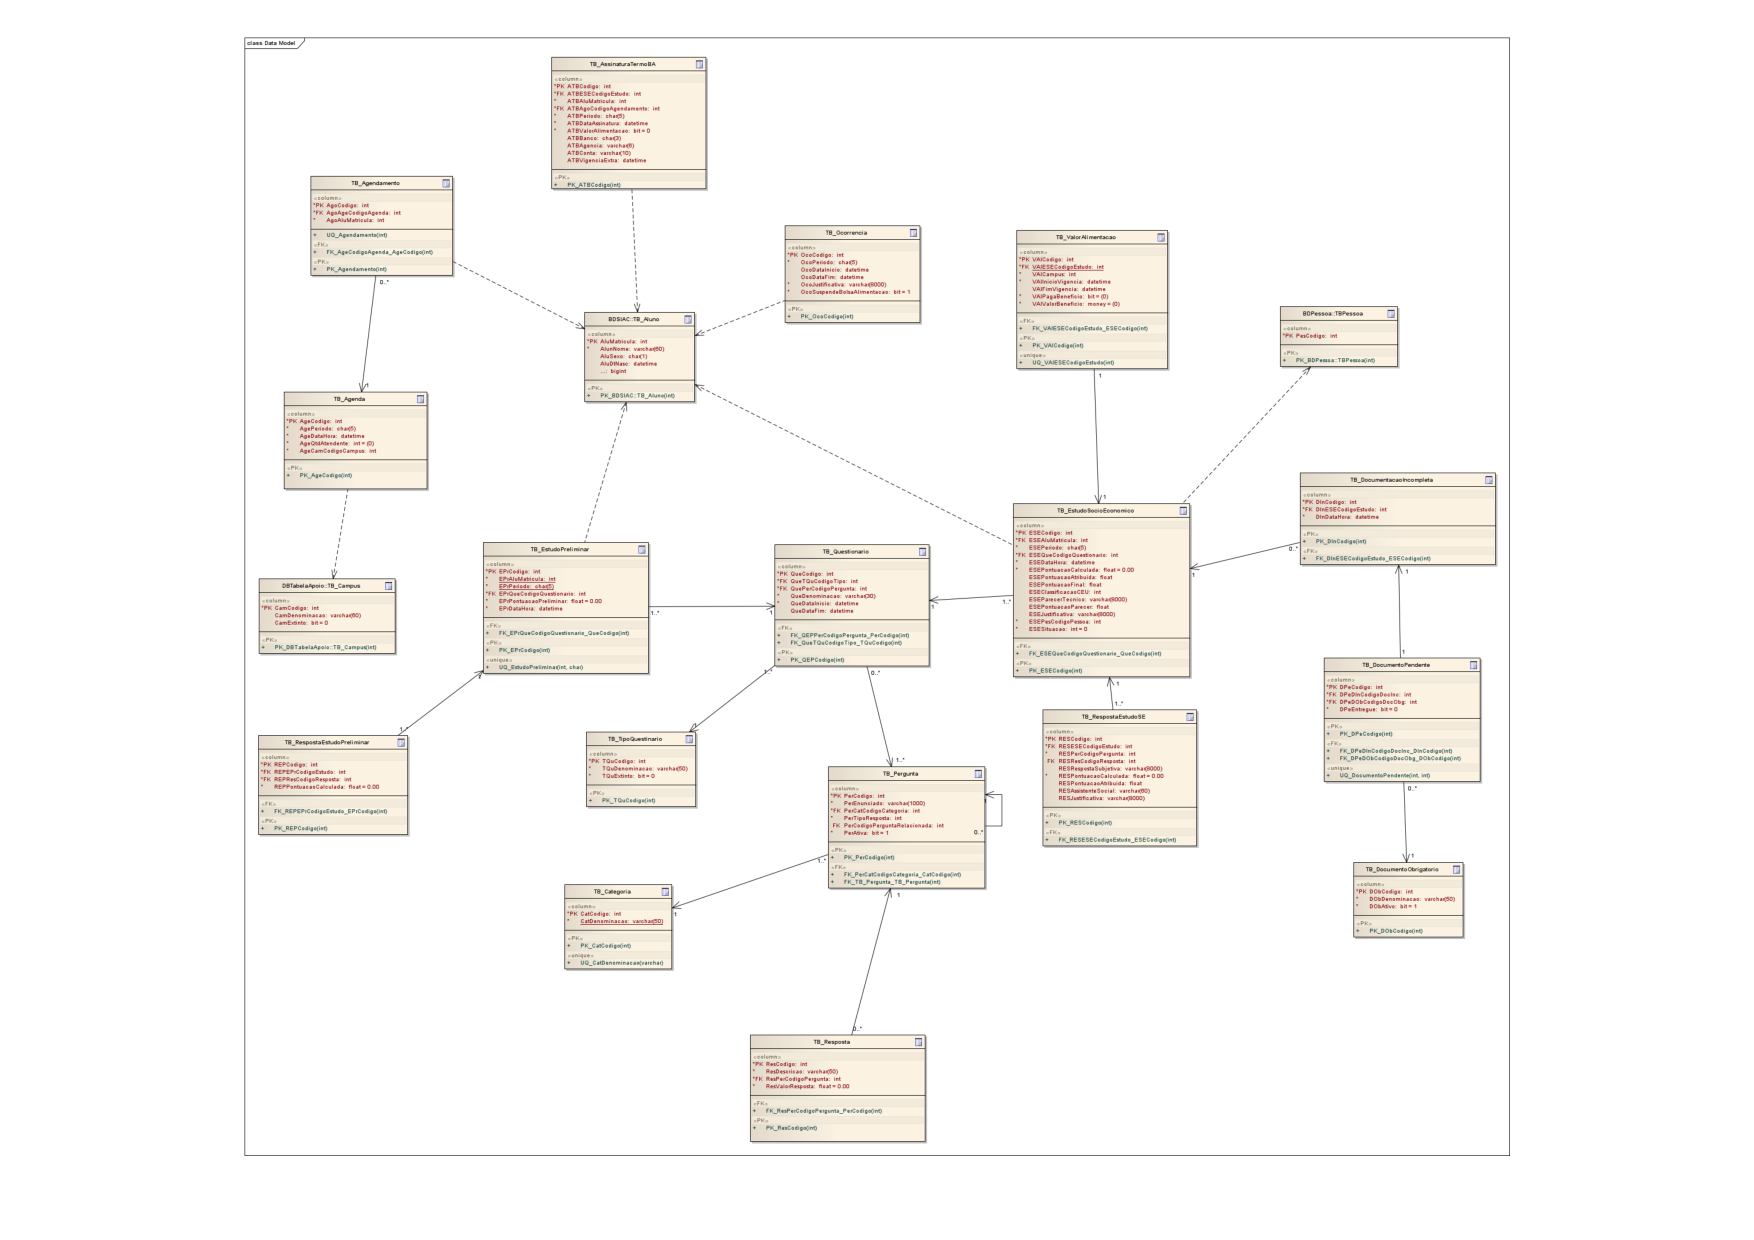
\includegraphics[scale=0.8]{img/sae.pdf}
\caption{Modelo Entidade Relacionamento (MER) do SAE.}
\label{fig:ER_SAE}
\end{figure}

